



\section{Introduction}
\vspace{-0.5em}
% The Illusion of Progress
Multimodal Large Language Models (MLLMs) have rapidly advanced video understanding~\cite{DBLP:conf/emnlp/LinYZCNJ024, DBLP:conf/acl/0001RKK24, DBLP:journals/tmlr/ZhangWLLMLL25}. Powered by foundation models such as GPT~\cite{DBLP:journals/corr/abs-2601-03267}, Gemini~\cite{deepmind2026gemini3}, and Qwen-VL~\cite{DBLP:journals/corr/abs-2511-21631}, recent Video-LLMs~\cite{DBLP:conf/nips/Dai0LTZW0FH23, zhang-etal-2023-video, Li2023VideoChatCV, DBLP:journals/corr/abs-2504-10479} can interpret dynamic scenes~\cite{Fu2024BLINKML, Ren2024Location}, answer complex questions~\cite{patraucean2023perception,Li2024MVBench}, and follow instructions~\cite{Wang2024InternVideo2SV,jin2023chatunivi}. 
Yet, in videos with both visual and acoustic signals, such capabilities can blur the boundary between genuine audio-visual grounding and visually driven narration. % such capability can conflate audio-visual grounding with visual narration: 
For example, when shown a skateboarder crashing onto concrete, a model may describe a heavy thud even when the audio evidence is absent or misaligned~\cite{DBLP:conf/emnlp/LiDZWZW23,DBLP:conf/cvpr/GuanLWXLL0CHYM024,sung-bin2025avhbench,Cai2025DiagnosingAM}.
Such behavior is often interpreted as multimodal perception, but it may instead reflect an illusion of audio-visual understanding: the model predicts what a video should sound like from what it sees. 
While static vision-language models are known to behave like ``bags-of-words'' driven by text priors~\cite{DBLP:conf/cvpr/Tong0Z0LX24, DBLP:conf/cvpr/ThrushJBSWKR22, DBLP:conf/iclr/Yuksekgonul0KJ023}, analogous prediction shortcuts in dynamic audio-visual contexts remain underexplored. This raises a central question: \textit{Are current video-capable multimodal models truly performing audio-visual grounding, or merely hallucinating acoustic events from visual-semantic shortcuts?}

\begin{tcolorbox}[
colback=bluegray!4,
colframe=bluegray!35,
boxrule=0.5pt,
arc=2pt,
left=6pt,
right=6pt,
top=3pt,
bottom=3pt,
title=\textbf{Clever Hans Effect in Audio-Visual Grounding},
fonttitle=\small,
coltitle=black
]
\looseness-3
\small
A video-capable multimodal model exhibits a \textit{Clever Hans effect} when it appears audio-grounded but produces sound-related outputs primarily from visual cues rather than verified audio evidence.
\end{tcolorbox}

\begin{figure}[t]
    \centering
    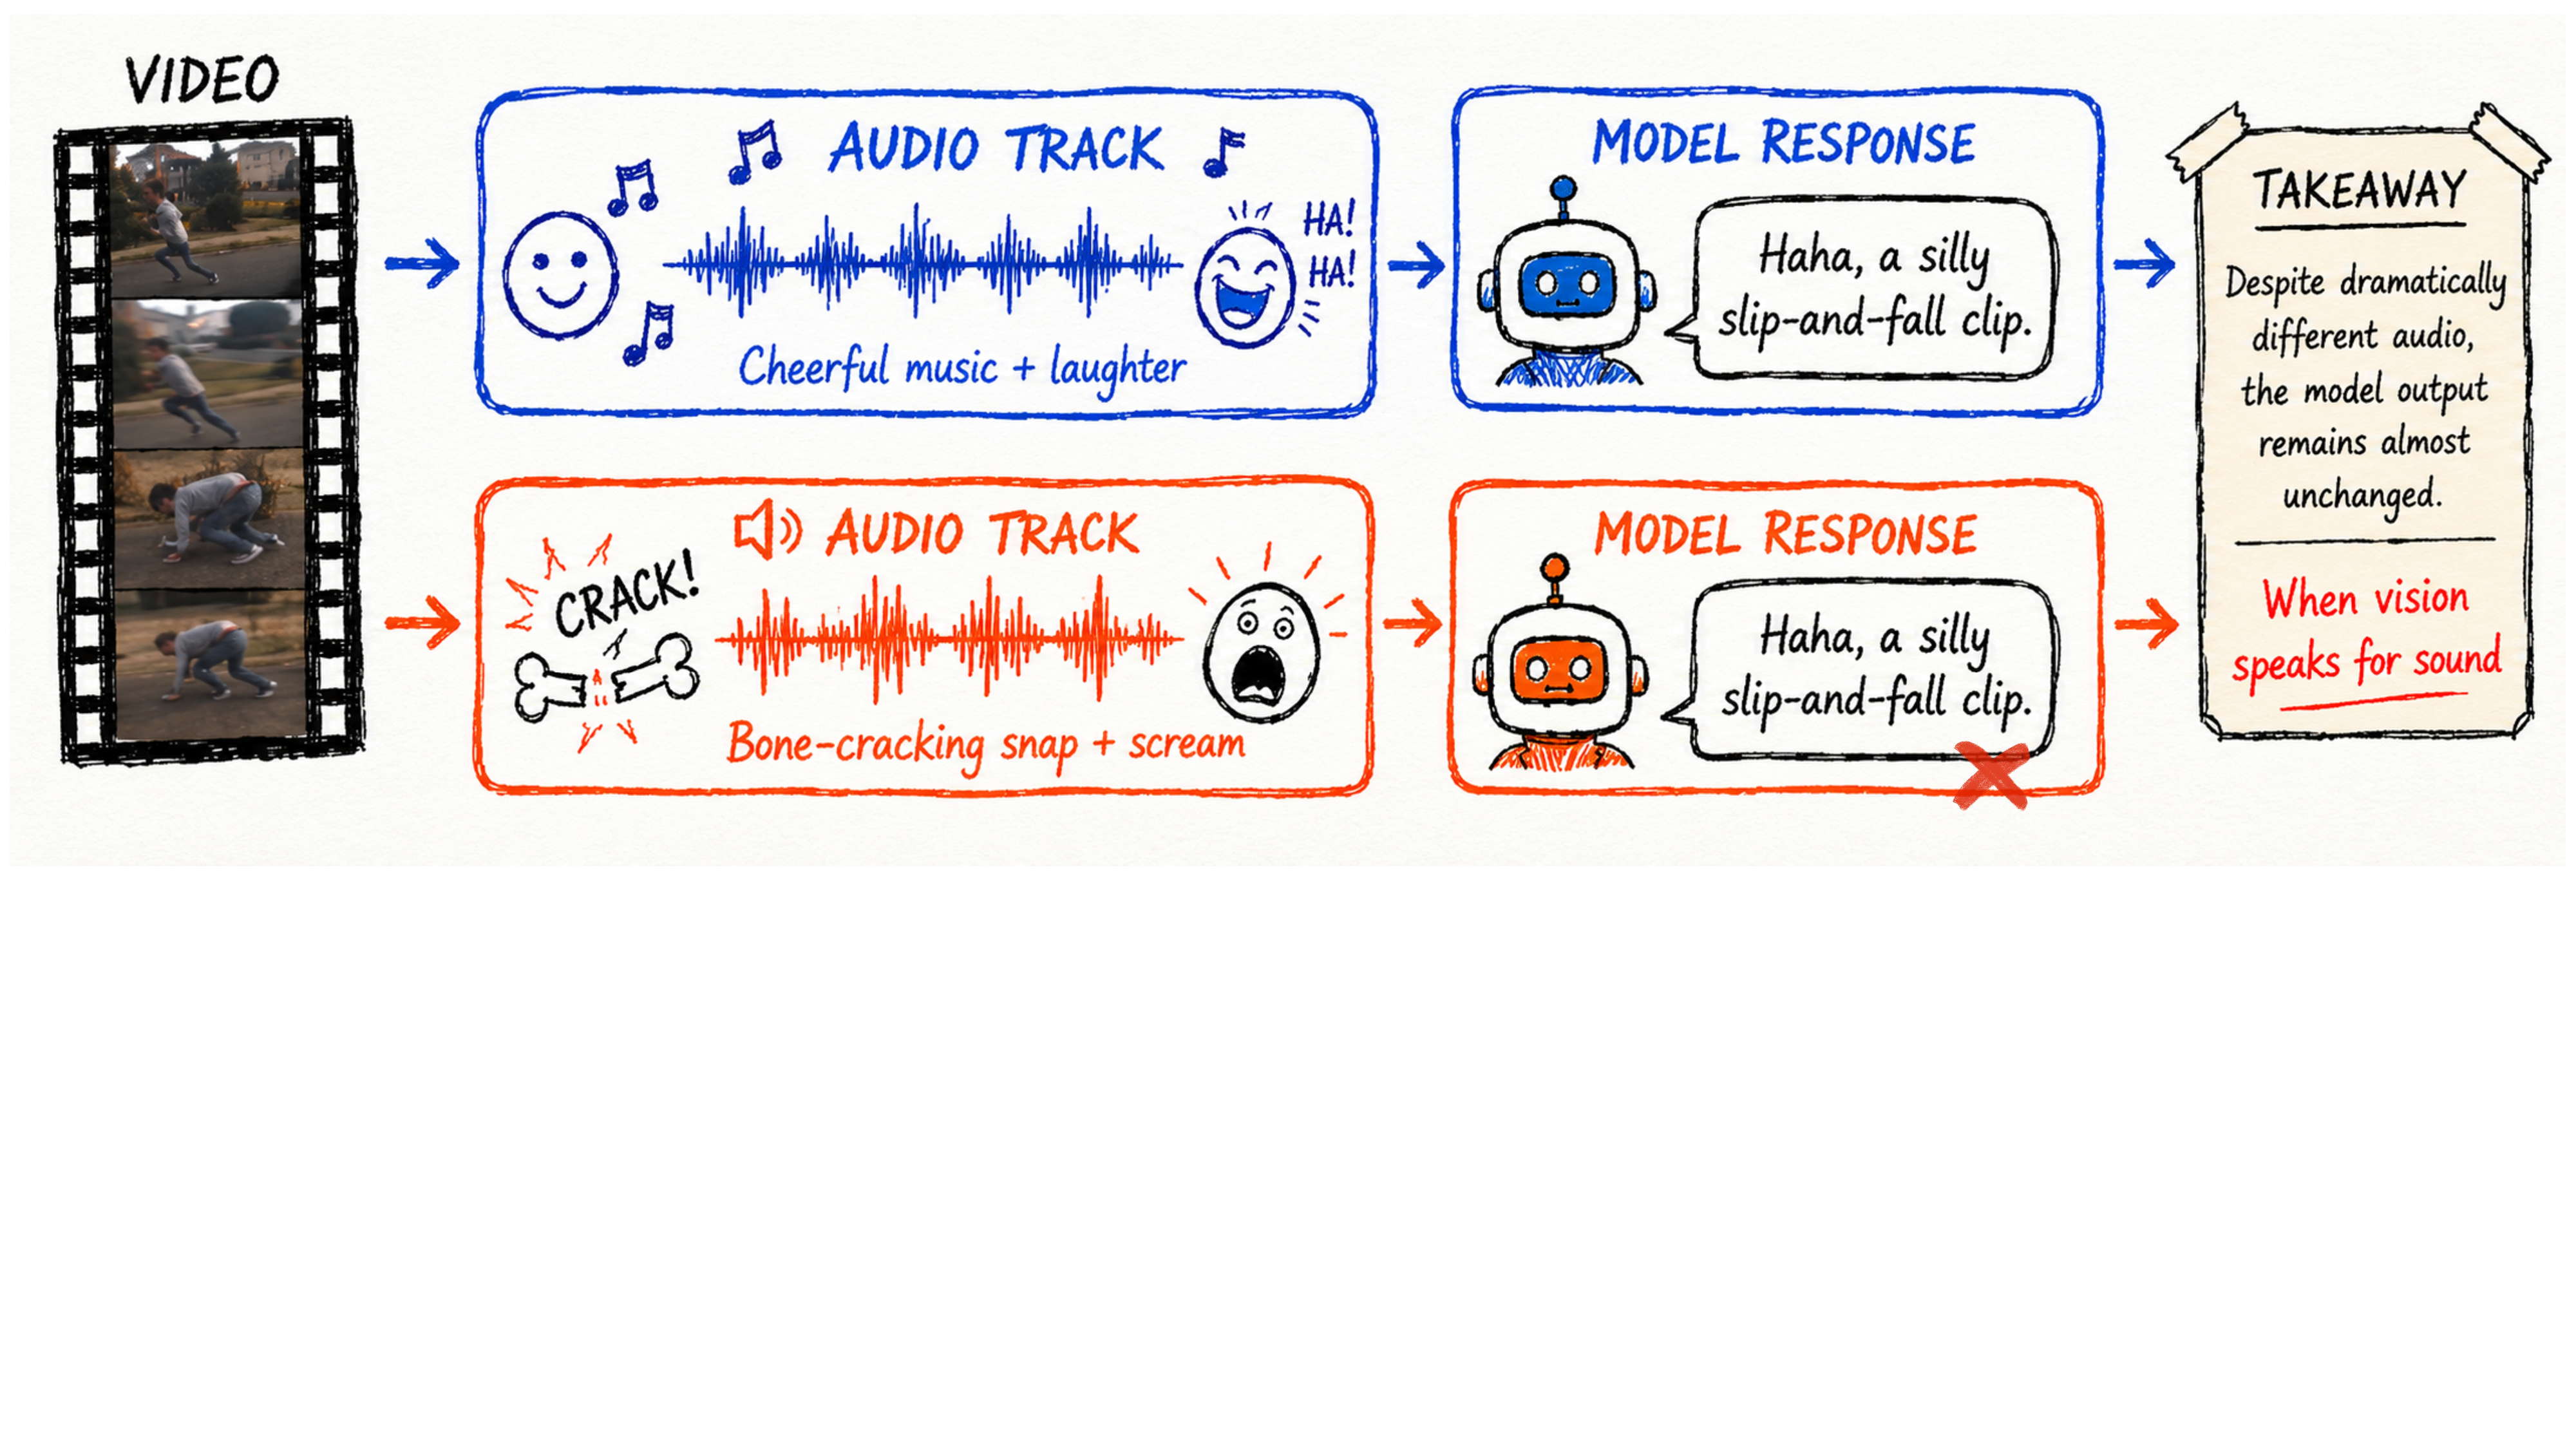
\includegraphics[width=\linewidth]{Fig/motivation_fig_3.pdf}

    \caption{
\textcolor{failurered}{\textbf{When vision speaks for sound}}.
Given the same visual event but different audio tracks, current video-capable models produce nearly identical captions, suggesting visual-prior shortcutting rather than audio-grounded understanding.
}
\vspace{-1cm}

    \label{fig:motivation}

\end{figure}

% \vspace{-0.3em}

\looseness-1
We find that current video-capable MLLMs are often visually dominated when reasoning about audio-related information in sounded videos. As illustrated in \Cref{fig:motivation}, this shortcut can lead models to produce nearly unchanged descriptions even when the audio track changes substantially. This behavior resembles the famous \textit{Clever Hans effect}~\cite{pfungst1911clever}, where apparent competence arises from exploiting unintended but correlated cues rather than performing the intended task. Such semantic laziness~\cite{DBLP:journals/natmi/GeirhosJMZBBW20} allows models to exploit visual-semantic shortcuts and language priors instead of fine-grained audio-visual grounding that checks whether the audio and visual streams are temporally and semantically consistent~\cite{DBLP:conf/iclr/Yuksekgonul0KJ023, DBLP:conf/cvpr/GoyalKSBP17}. This failure often remains hidden because common audio-visual evaluations preserve the natural correlations that make such shortcuts effective~\cite{Gemmeke2017AudioSA,Chen2020VggsoundAL,Carreira2017QuoVA}: barking dogs produce barks, falling objects produce impacts, and speaking faces produce speech~\cite{Arandjelovi2017LookLA,Owens2018AudioVisualSA}. As a result, a model can appear grounded by recognizing the visual event and predicting its likely sound, without verifying whether that sound is actually present, synchronized, or physically consistent. This pseudo-alignment creates an illusion of multimodal understanding that current evaluations often fail to expose~\cite{DBLP:conf/nips/MangalamAM23,DBLP:conf/cvpr/0002WH00LWX0L0024}. To expose the Clever Hans effect, evaluation must move beyond naturally correlated videos and use controlled interventions that systematically break the audio-visual correspondences that allow visual-semantic shortcuts to succeed~\cite{Korbar2018CooperativeLO,Morgado2020AudioVisualID}.

To this end, we introduce \textbf{\Thud}~(\textbf{T}emporal and \textbf{H}allucination \textbf{U}nmasking \textbf{D}iagnostics), an intervention-driven diagnostic protocol for probing audio-visual grounding in sounded videos. \Thud~constructs a dynamic probing space by counterfactually perturbing the audio-visual correspondences of natural videos across temporal synchronization, audio existence, and sound consistency, thereby neutralizing semantic shortcuts and exposing whether a model engages in genuinely grounded audio-visual reasoning or merely hallucinates from visual-semantic and language priors. Beyond diagnosis, we further study whether targeted post-training can mitigate these shortcuts through a family of alignment recipes that combine intervention-derived preference pairs with general video data. The best-performing recipe uses a 10K-sample mixture of counterfactual temporal preferences and event-level general video supervision, substantially improving the model's ability to detect temporal interventions, including out-of-distribution synchronization tests, while avoiding an alignment tax~\cite{Askell2021AGL,DBLP:conf/nips/Ouyang0JAWMZASR22} on standard video understanding benchmarks. 
Additional targeted supervision on Mute and Swap further improves audio-existence and sound-consistency verification, showing that intervention-based training can be extended beyond temporal alignment.
However, the same training yields only marginal gains without such targeted examples, suggesting that temporal synchronization, audio existence, and sound consistency are distinct failure modes of grounded audio-visual understanding rather than a single unified deficiency.

% Specifically, we introduce temporal \textit{Shift} to the sound to evaluate strict temporal synchronization, apply \textit{Mute} to the audio track to assess sound-presence hallucinations, and leverage acoustic \textit{Swap} to test whether models can verify semantic and physical consistency between the visual event and the accompanying sound.
% By forcing models into these counterfactual corners, \Thud~effectively neutralizes semantic shortcuts and exposes whether a model is engaging in genuinely grounded audio-visual reasoning or merely hallucinating based on visual-semantic and language priors.

% The Cure and the Orthogonal Discovery
% Beyond diagnosis, we further study whether targeted post-training can mitigate these shortcuts through a family of alignment recipes that combine intervention-derived preference pairs with general video data. The best-performing recipe uses a 10K-sample mixture of counterfactual temporal preferences and event-level general video supervision, substantially improving the model's ability to detect \textit{Shift} interventions, including out-of-distribution synchronization tests, while avoiding an alignment tax~\cite{Askell2021AGL,DBLP:conf/nips/Ouyang0JAWMZASR22} on standard video understanding benchmarks. However, the same training yields only marginal gains on \textit{Mute} and \textit{Swap}, suggesting that \textit{temporal synchronization}, \textit{audio existence}, and \textit{sound consistency} distinct failure modes of grounded audio-visual understanding rather than a single unified deficiency.

% However, it also exposes an important limitation: despite improved temporal anchoring, the model shows only marginal gains on \textit{Mute} and \textit{Swap} interventions. This finding suggests that \textit{temporal synchronization} and \textit{existential verification} are empirically separable dimensions of audio-visual grounding. Improving a model's ability to align events in time does not automatically enable it to verify whether a sound exists or whether it is physically consistent with the visual scene, revealing a key blind spot in current multimodal alignment.

In summary, we make three contributions:
1) We identify and systematically expose a \textit{Clever Hans} effect in current Video-LLMs, where models substitute genuine audio-visual grounding with visual-semantic shortcuts. Through controlled interventions, we quantify how strongly models rely on visual priors when answering sound-related questions.
2) We introduce \Thud, a counterfactual diagnostic protocol that dismantles natural cross-modal correlations. By applying \textit{Mute}, \textit{Shift}, and \textit{Swap} interventions, \Thud{} audits existential, temporal, and material aspects of audio-visual grounding.
3) We evaluate preference-optimization recipes for mitigating audio-visual shortcuts. Our final 10K recipe improves average performance across \textit{Shift}, \textit{Mute}, and \textit{Swap} interventions by 28\%, while slightly improving general video and audio-visual understanding.

% Contributions
% In summary, our contributions are three-fold:
% \begin{itemize}[leftmargin=1.5em, itemsep=4pt, topsep=4pt, parsep=0pt]
%     \item We identify and systematically expose a \textit{Clever Hans} effect in current Video-LLMs, where models can substitute genuine audio-visual grounding with visual-semantic shortcuts. Through controlled interventions, we quantify how strongly these models rely on visual priors when answering sound-related questions.
    
%     \item We introduce \Thud, a counterfactual diagnostic protocol that systematically dismantles natural cross-modal correlations. By applying \textit{Mute}, \textit{Shift}, and \textit{Swap} interventions, \Thud{} forces models into counterfactual settings that explicitly audit existential, temporal, and material aspects of audio-visual grounding.
    
%     \item We evaluate a family of preference-optimization recipes for mitigating audio-visual shortcuts. Our final 10K recipe improves average performance across \textit{Shift}, \textit{Mute}, and \textit{Swap} interventions by 28\%, while slightly improving general video understanding and audio-visual understanding.
% \end{itemize}
